\documentclass[uplatex,dvipdfmx,a4paper,11pt]{jsarticle}

\usepackage[dvipdfmx]{graphicx}
\usepackage[dvipdfmx]{hyperref}
\usepackage{amsmath}
\usepackage{booktabs}
\usepackage{array}
\usepackage{longtable}
\usepackage{url}
\usepackage{geometry}
\usepackage{xcolor}
\geometry{margin=22mm}

\hypersetup{
  colorlinks=true,
  linkcolor=blue,
  citecolor=blue,
  urlcolor=blue
}

\graphicspath{{figures/}{../results/}}

\title{カテゴリ別プロファイル型PatchCore-liteのFPGA実装に向けた説明資料}
\author{山田 俊介}
\date{2026年8月23日}

\begin{document}
\maketitle

\section*{概要}

本資料では，検品向け異常検知手法であるPatchCoreを題材に，
「単にPatchCoreをFPGAに載せる」のではなく，
検品対象カテゴリごとに必要なメモリバンクとKNN探索量を事前に決定し，
その構成をFPGA上で切り替える方式を提案する。

現在までの実験から，PatchCoreの重い部分であるKNN探索は平均で
基準構成の0.0109倍，中央値で0.0035倍まで削減できる見込みが得られた。
また，全15カテゴリ分のメモリバンクを保持する場合でも，
カテゴリ別に選択した構成では131.660 MiBから3.288 MiBへ削減できる。
一方で，15カテゴリすべてに対して厳しい検品品質を同時に満たすことは
現時点では難しく，初回実装はhazelnutなど成立しやすいカテゴリに絞るのが妥当である。

\section{PatchCoreとは}

\subsection{検品タスクにおける位置づけ}

PatchCoreは，工業製品の外観検査で用いられる異常検知手法である。
通常の画像分類モデルは，良品画像と欠陥画像の両方を用いて
「どのクラスか」を学習する。一方，実際の検品現場では，
欠陥品の種類が多く，そもそも欠陥画像を十分に集められない場合がある。
PatchCoreはこの状況に対し，
正常画像のみを用いて「正常らしさ」を記憶し，
検査画像がその正常分布からどれだけ離れているかを測る。

PatchCoreの元論文では，MVTec ADにおいて高い画像レベル異常検知性能を示しており，
特に欠陥例が少ない cold-start な検品タスクに強いことが特徴である
\cite{patchcore_cvpr}。MVTec ADは15種類の工業検品カテゴリを含む
代表的な異常検知ベンチマークであり，正常学習画像と正常/異常のテスト画像を持つ
\cite{mvtec_ad}。

\subsection{基本動作}

PatchCoreの処理は大きく2段階に分かれる。

\begin{enumerate}
  \item \textbf{準備段階}: 正常画像をCNN特徴抽出器に通し，画像内の局所特徴をパッチ特徴として取り出す。
  その正常パッチ特徴をメモリバンクに保存する。
  \item \textbf{推論段階}: 検査画像から同様にパッチ特徴を取り出し，
  各パッチ特徴に対してメモリバンク内の最近傍特徴をKNN探索で探す。
  近い正常特徴が見つからないほど異常スコアが高くなる。
\end{enumerate}

\begin{figure}[t]
  \centering
  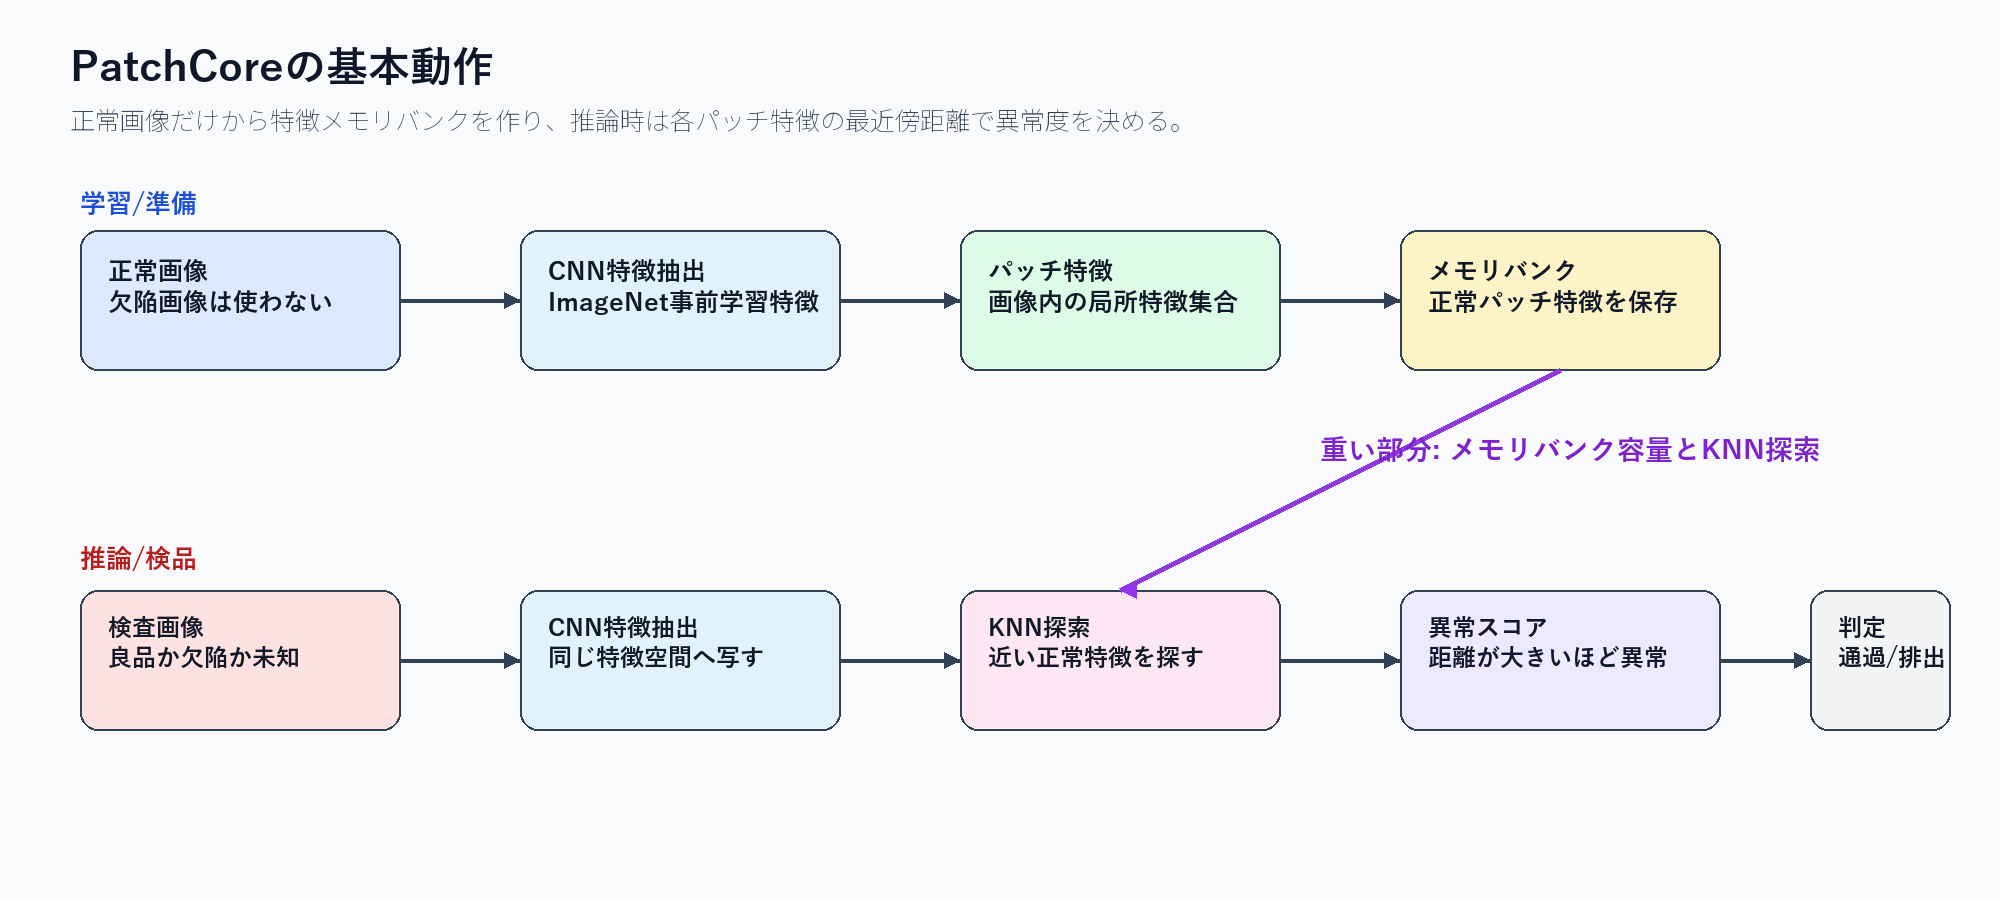
\includegraphics[width=\linewidth]{patchcore_flow.png}
  \caption{PatchCoreの基本動作。重い部分はメモリバンク容量とKNN探索である。}
  \label{fig:patchcore-flow}
\end{figure}

重要な用語は以下の通りである。

\begin{description}
  \item[パッチ特徴]
  画像全体を1つの特徴に潰すのではなく，画像内の局所領域ごとに取り出した特徴である。
  局所的な傷や汚れを検出しやすい。

  \item[メモリバンク]
  正常画像から得られたパッチ特徴の集合である。
  推論時には，検査画像のパッチ特徴がこの正常特徴集合にどれだけ近いかを見る。

  \item[KNN探索]
  検査画像の各パッチ特徴について，メモリバンク内の近い特徴を探す処理である。
  PatchCoreの精度を支える一方，計算量とメモリアクセス量が大きい。

  \item[異常スコア]
  検査画像のパッチ特徴と正常メモリバンクの距離から計算される値である。
  スコアが高いほど「正常から離れている」と判断する。
\end{description}

\subsection{強みと弱み}

PatchCoreの強みは，欠陥画像を大量に用意しなくても検品タスクを構成しやすい点である。
また，画像全体の分類ではなく局所パッチ特徴を使うため，傷や汚れの位置をある程度反映できる。
CNN分類器やU-Net系の教師あり検査モデルと比べると，
欠陥ラベルへの依存が小さい。

一方で，弱みは明確である。
メモリバンクを大きくすると正常特徴を細かく保持できるが，
メモリ容量とKNN探索量が増える。
KNN探索の概算演算量は，
\[
  C_{\mathrm{KNN}} \propto N_{\mathrm{patch}} \times N_{\mathrm{bank}} \times D
\]
で表せる。ここで，$N_{\mathrm{patch}}$は検査画像から得られるパッチ数，
$N_{\mathrm{bank}}$はメモリバンク中の正常パッチ特徴数，
$D$は特徴次元数である。したがって，
特徴層，パッチグリッド，バンクサイズの選び方が実装コストに直結する。

\section{カテゴリを絞れば削減できる根拠}

\subsection{実験の目的}

今回の実験では，MVTec ADの15カテゴリを対象に，
PatchCoreの構成をどこまで削減できるかを調べた。
ここで重要なのは，単に平均AUROCを見るのではなく，
検品タスクとして以下を分けて評価した点である。

\begin{itemize}
  \item \textbf{欠陥誤通過}: 欠陥品を良品として通してしまう割合。
  \item \textbf{良品通過}: 良品を良品として通せる割合。
  \item \textbf{KNN演算量}: メモリバンク探索に必要な相対演算量。
  \item \textbf{メモリバンク量}: FPGA上で保持すべき特徴量の相対サイズ。
\end{itemize}

検品では欠陥誤通過が特に重要である。
そのため，AUROCだけが高くても，固定閾値で欠陥誤通過を十分抑えられなければ
実用上は不十分である。

\subsection{全カテゴリ共通設定との比較}

まず，全カテゴリで同じ軽量構成を使う場合を調べた。
その結果，KNN演算量を20\%以下に抑えた共通構成では，
良品通過は57.19\%，KNN演算量は0.1667倍であった。
さらにKNN演算量を10\%以下に抑えると，良品通過は44.88\%まで低下した。
これは，カテゴリごとに必要な特徴層やバンク量が異なるため，
一つの共通軽量設定ですべてを処理するのは不利であることを示している。

\begin{table}[t]
  \centering
  \caption{全カテゴリ共通設定とカテゴリ別選択設定の比較}
  \label{tab:uniform-vs-profiled}
  \begin{tabular}{p{65mm}rrp{55mm}}
    \toprule
    設定 & 良品通過 & KNN演算 & 読み取り \\
    \midrule
    全カテゴリ共通: 基準構成 & 59.34\% & 1.0000倍 & 最も重い参照点 \\
    全カテゴリ共通: KNN 20\%以下 & 57.19\% & 0.1667倍 & 共通軽量化で品質を残せる限界の目安 \\
    全カテゴリ共通: KNN 10\%以下 & 44.88\% & 0.0834倍 & さらに軽くすると良品通過が大きく下がる \\
    カテゴリ別選択設定，holdout平均 & 54.59\% & 0.0206倍 & KNNは非常に小さいが，品質はカテゴリ別に扱う必要がある \\
    \bottomrule
  \end{tabular}
\end{table}

\subsection{カテゴリ別プロファイルの結果}

次に，カテゴリごとに特徴層，パッチグリッド，バンクサイズ，閾値を選択した。
このカテゴリ別プロファイルにより，KNN探索コストは平均0.0109倍，
中央値0.0035倍となった。また，CNN特徴抽出とKNN探索を合わせた総コスト近似でも，
平均0.2687倍，中央値0.2035倍であった。

\begin{figure}[t]
  \centering
  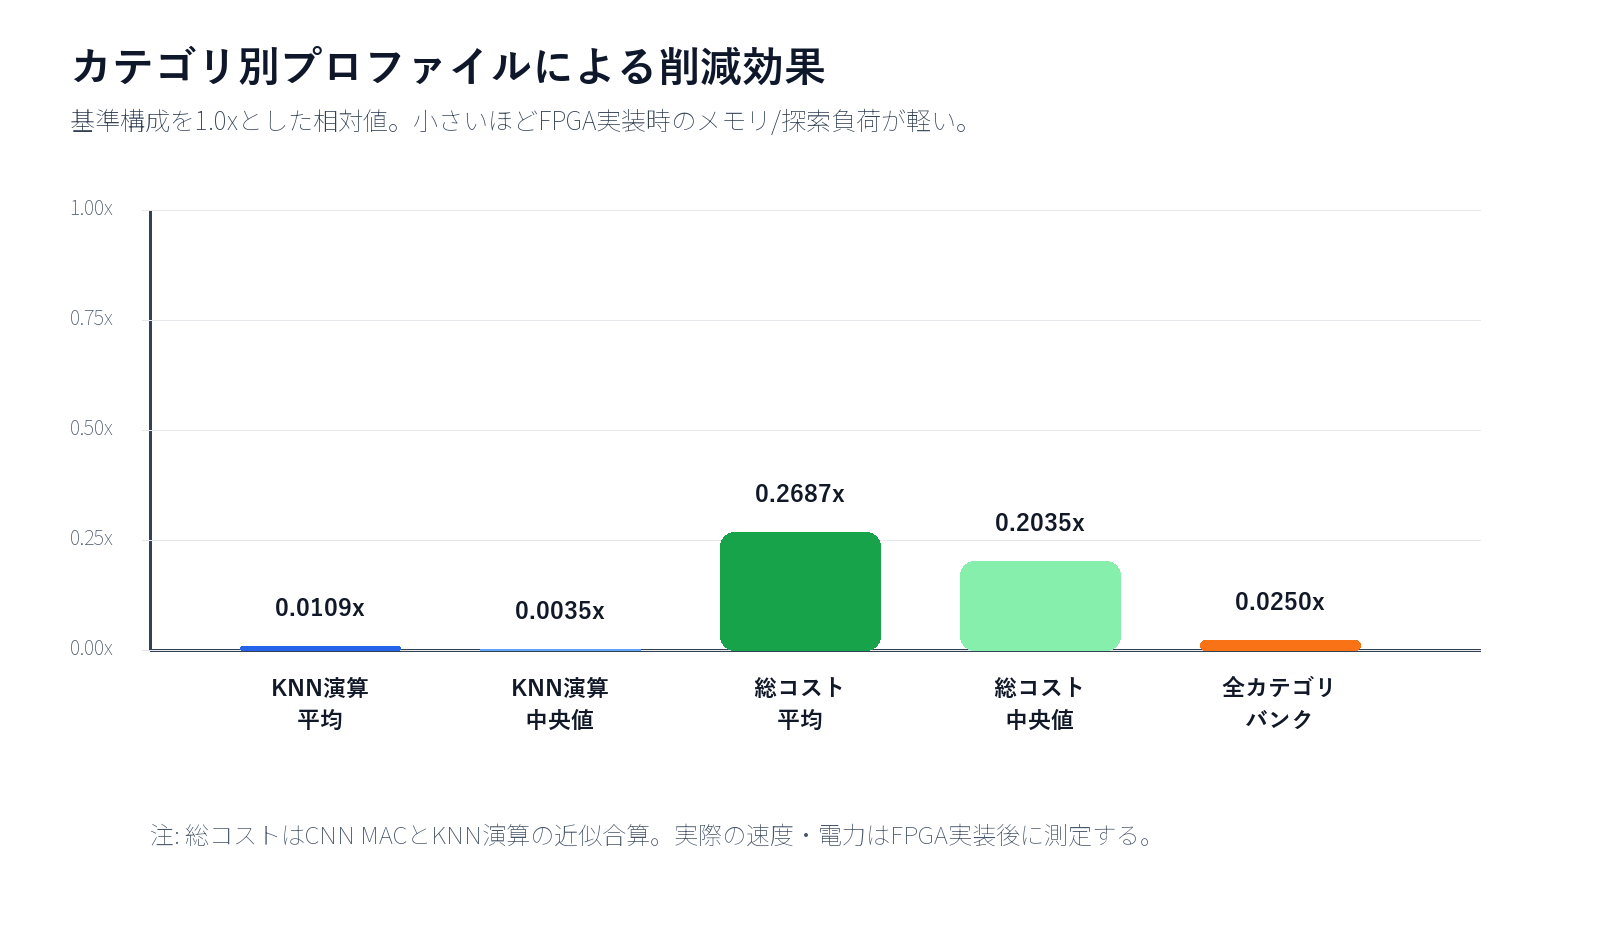
\includegraphics[width=.92\linewidth]{profiled_reduction_bars.png}
  \caption{カテゴリ別プロファイルによる削減効果。基準構成を1.0倍とした相対値。}
  \label{fig:reduction-bars}
\end{figure}

全カテゴリ分のメモリバンクを単純に基準構成で保持すると131.660 MiBが必要である。
一方，カテゴリ別に選択したバンクだけを保持する場合は3.288 MiBとなり，
常駐メモリは約97.50\%削減できる。
また，512並列の距離計算器を仮定したKNNレイテンシモデルでは，
平均0.193 ms，最大1.470 msという見積もりになった。

\subsection{品質面の限界}

ただし，全15カテゴリで厳しい検品品質を満たせたわけではない。
選択済みプロファイル設定が欠陥誤通過3\%以下を満たしたのは5/15カテゴリ，
5\%以下では9/15カテゴリであった。
したがって，現時点で主張すべきことは
「全カテゴリに対して万能に安全な軽量PatchCoreを得た」ではない。

主張すべきことは，
\begin{quote}
検品対象カテゴリが事前に分かる場合，
そのカテゴリに必要な特徴層・バンク量・探索量だけを選ぶことで，
FPGA実装に向いた小さい構成を作れる。
\end{quote}
という点である。

\begin{table}[t]
  \centering
  \caption{初回FPGA実装の候補}
  \label{tab:first-targets}
  \begin{tabular}{llrrrr}
    \toprule
    カテゴリ & 選択設定 & 良品通過 & 欠陥誤通過 & 総コスト近似 & KNN演算 \\
    \midrule
    hazelnut & res18\_l23\_g14\_b500 & 92.00\% & 1.14\% & 0.1008倍 & 0.0104倍 \\
    zipper & wrn\_l3\_g14\_b1500 & 75.00\% & 2.71\% & 0.5220倍 & 0.0833倍 \\
    wood & res18\_l23\_g7\_b125 & 71.11\% & 2.00\% & 0.0957倍 & 0.0007倍 \\
    cable & res18\_l23\_g7\_b1500 & 33.79\% & 2.61\% & 0.0995倍 & 0.0078倍 \\
    \bottomrule
  \end{tabular}
\end{table}

初回実装としては，良品通過92.00\%，欠陥誤通過1.14\%，
総コスト近似0.1008倍のhazelnutが最も扱いやすい。
woodやcableは，より小さい構成を試す比較対象として有用である。

\section{目指す提案システム}

\subsection{基本方針}

提案システムは，リアルタイムに画像ごとに複雑なルーティングを行う方式ではない。
検品ラインでは，通常，その時間帯に検査する製品カテゴリは事前に分かっている。
そこで，検品動作の前にカテゴリを選択し，
そのカテゴリに対応するPatchCore-lite構成をFPGA上で有効化する。

具体的には，カテゴリごとに以下を事前に決める。

\begin{itemize}
  \item 使用するCNN特徴層
  \item パッチグリッドサイズ
  \item メモリバンクサイズ
  \item 異常判定閾値
  \item 距離計算器に流す特徴次元とバンク配置
\end{itemize}

\begin{figure}[t]
  \centering
  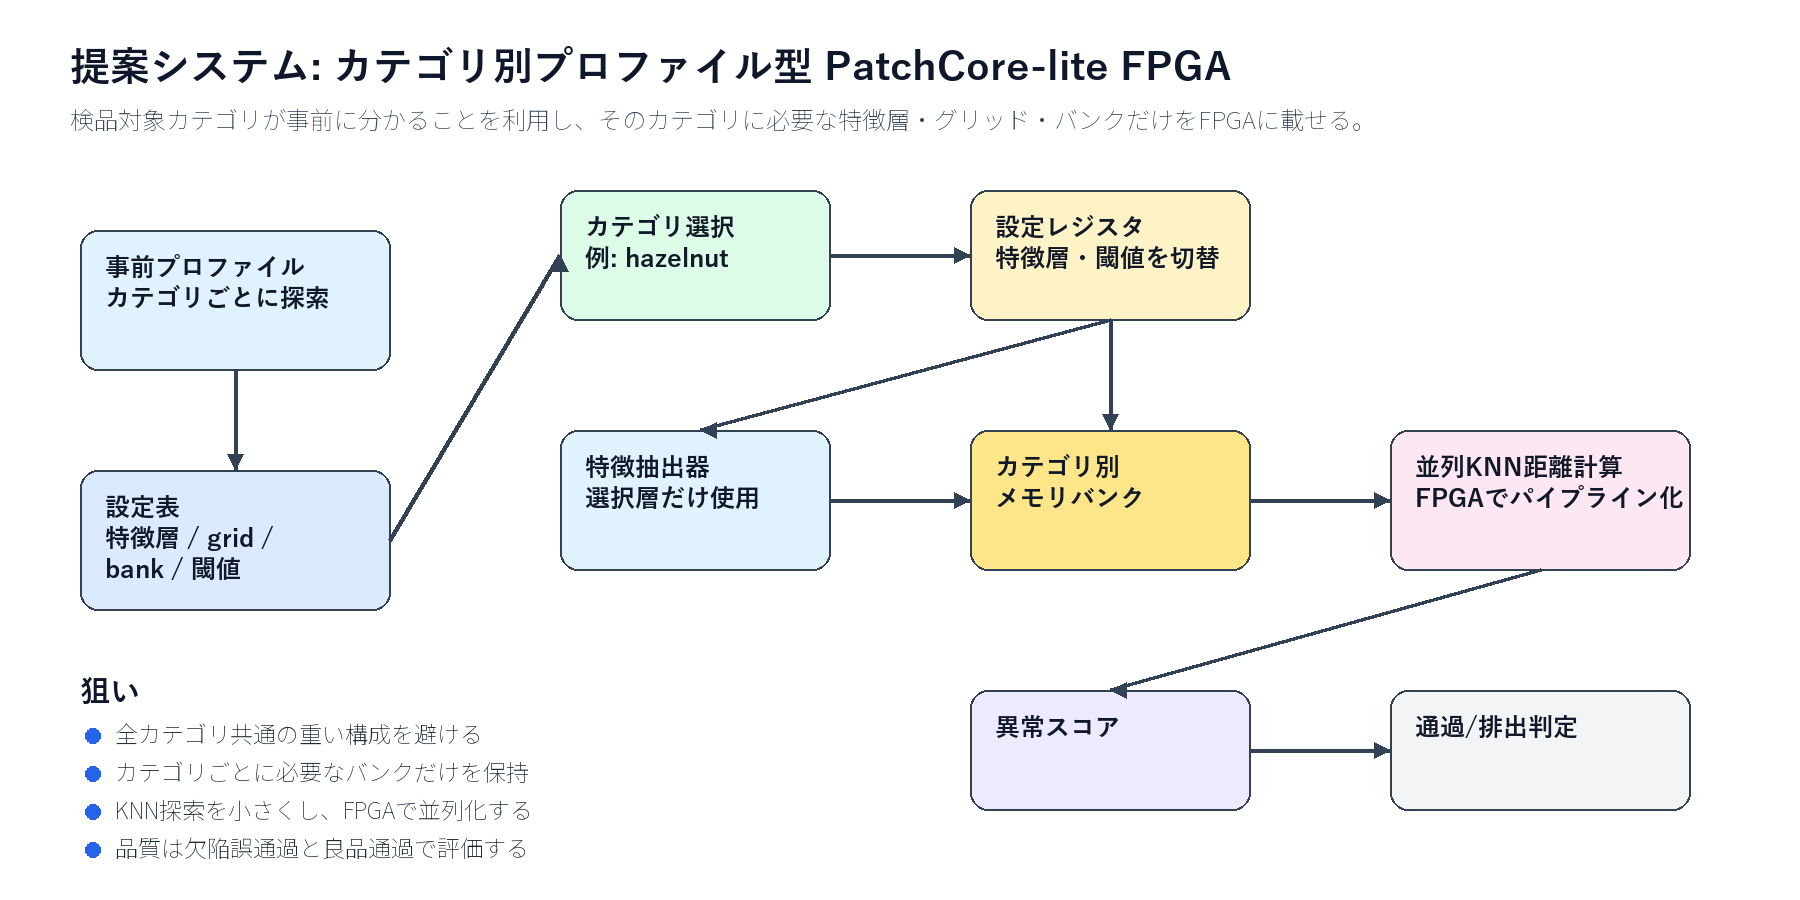
\includegraphics[width=\linewidth]{proposed_patchcore_fpga.png}
  \caption{提案するカテゴリ別プロファイル型PatchCore-lite FPGA構成。}
  \label{fig:proposed-system}
\end{figure}

\subsection{動作イメージ}

例えばhazelnutを検査する時間帯には，hazelnut用に選択した
特徴抽出設定，メモリバンク，閾値を読み込む。
検査中はその設定で固定動作し，入力画像ごとに異常スコアを計算する。
別カテゴリに切り替える場合は，検品前に設定レジスタとメモリバンクを切り替える。

この方式は，画像ごとに複雑な判断器を走らせるのではなく，
「検品対象カテゴリが既知である」という工業検品の前提を利用する。
したがって，動的切り替えというよりは，
カテゴリ別の実行モードを持つFPGAアクセラレータである。

\section{既存手法に対する優位性}

\subsection{通常のPatchCoreに対して}

通常のPatchCoreは高精度である一方，メモリバンクとKNN探索が重い。
本研究の提案は，PatchCoreの検出原理そのものを変えるのではなく，
検品対象ごとに必要な特徴量とメモリバンクだけを残し，
FPGA実装可能な形に縮約する点にある。

単なる軽量化と異なる点は，
全カテゴリ共通に同じ小型構成を使うのではなく，
カテゴリごとに良品通過と欠陥誤通過を見ながら構成を選ぶ点である。
これは，検品では平均精度よりも，
対象製品ごとの誤通過率と通過率が重要になるためである。

\subsection{分類器・セグメンテーション器に対して}

通常のCNN分類器やU-Net系のセグメンテーション器は，
欠陥画像と欠陥ラベルが十分に用意できる場合には強力である。
しかし，実際の検品では未知欠陥や少数欠陥が問題になりやすい。
PatchCore系は正常画像のみから正常分布を作るため，
欠陥データ収集コストが高い状況に向いている。

したがって，本研究の位置づけは，
教師あり検品器を置き換えるというより，
欠陥例が少ない検品対象に対して，
正常画像ベースの異常検知をFPGA上で実行しやすくすることである。

\subsection{カスケード方式・パラレル方式・早期終了方式に対して}

これまで検討したカスケード方式，パラレル方式，BranchyNet型早期終了
\cite{branchynet} は，主に画像分類モデルの推論を途中で切り替える考え方である。
しかし，検品タスクでは「高信頼の分類ラベルを早く出す」だけでは不十分であり，
欠陥誤通過を抑えたうえで良品通過をどこまで確保できるかが重要になる。

本提案は，画像ごとの分岐判断を主張の中心に置かない。
代わりに，検品対象カテゴリが事前に分かるという前提を使い，
そのカテゴリに必要なメモリバンクとKNN探索量を設計時に決める。
このため，分岐予測器の失敗や画像ごとの実行時間ばらつきではなく，
固定されたモードごとの資源量とレイテンシを評価しやすい。

\subsection{既存のPatchCore高速化・FPGA化研究に対して}

PatchCoreの高速化やメモリ削減は既に研究されている。
例えば，メモリバンク圧縮や近似探索による高速化，
画像縮小や軽量バックボーンによる高速化が報告されている。
また，MAD-Flowはメモリバンク型異常検知をFPGA-SoCへ展開する
近い先行研究であり，メモリ容量とKNN探索遅延を主要課題として扱っている
\cite{madflow}。

したがって，本研究を
「PatchCoreをFPGAに載せた」
だけで主張するのは弱い。
本研究で狙うべき差分は以下である。

\begin{itemize}
  \item AUROCだけでなく，欠陥誤通過と良品通過を分けて評価する。
  \item カテゴリごとに特徴層・グリッド・バンク量を選ぶ。
  \item その選択結果をFPGAのメモリ量，距離計算並列度，レイテンシへ対応づける。
  \item 単一カテゴリ実装から，カテゴリモード切替型の複数カテゴリ対応へ拡張する。
\end{itemize}

この立て方であれば，既存の高速化研究を踏まえたうえで，
検品制約付きのFPGA向け設計最適化として主張できる。

\section{FPGA化で得られることと見積もり性能}

\subsection{FPGA化で効く部分}

PatchCoreのKNN探索は，同じ形の距離計算を多数のメモリバンク特徴に対して繰り返す。
この処理は，FPGA上で並列距離計算器として実装しやすい。
CPUやGPUでは汎用メモリ階層やバッチ処理の影響を受けるが，
FPGAでは以下を固定回路として設計できる。

\begin{itemize}
  \item メモリバンクのビット幅と配置
  \item 距離計算器の並列数
  \item ストリーミング入力に対するパイプライン処理
  \item 閾値比較による通過/排出判定
  \item カテゴリモード切替時のバンク選択
\end{itemize}

特に，カテゴリ別プロファイルによりバンクサイズを小さくできると，
必要なBRAM/URAM/外部メモリアクセス量が減り，
距離計算器の並列化も現実的になる。

\subsection{見積もり性能}

現在のコストモデルでは，以下の見積もりが得られている。

\begin{table}[t]
  \centering
  \caption{FPGA実装前の性能見積もり}
  \label{tab:fpga-estimate}
  \begin{tabular}{lrp{78mm}}
    \toprule
    項目 & 値 & 意味 \\
    \midrule
    KNN演算量平均 & 0.0109倍 & 距離探索の演算回数は約98.9\%削減 \\
    KNN演算量中央値 & 0.0035倍 & 多くのカテゴリではさらに小さい \\
    総コスト近似平均 & 0.2687倍 & CNN特徴抽出とKNN探索を合わせても削減が残る \\
    全カテゴリ分バンク & 3.288 MiB & 基準構成131.660 MiBから約97.5\%削減 \\
    512並列KNN平均 & 0.193 ms & 削減後バンクに対する距離探索レイテンシ見積もり \\
    512並列KNN最大 & 1.470 ms & 選択カテゴリ中の最大見積もり \\
    \bottomrule
  \end{tabular}
\end{table}

ただし，これは実装前のモデルであり，
実際の速度・電力・資源量はFPGA実装後に測定する必要がある。
特に，固定小数点化やint8/int4化により異常スコアの分布が変わる可能性がある。
したがって，実装後には以下を測定する。

\begin{itemize}
  \item 論理資源，BRAM/URAM，DSP使用量
  \item 実レイテンシとスループット
  \item 消費電力
  \item 固定小数点化前後の欠陥誤通過と良品通過
  \item ソフトウェア推定コストとFPGA実測値の差
\end{itemize}

\section{今後の作業}

実装前の追加GPU探索は一旦止め，以下の順で進める。

\begin{enumerate}
  \item hazelnutを対象に，選択済みPatchCore-lite構成を固定する。
  \item ソフトウェア側で同じ構成の入出力を固定し，FPGA実装の検証データを作る。
  \item KNN距離計算部をまずFPGA上に実装する。
  \item その後，特徴抽出部，メモリバンク配置，閾値判定を含めた全体構成へ拡張する。
  \item 実測値を用いて，コストモデルとの差，速度，電力，品質変化を評価する。
  \item 単一カテゴリで成立した後，カテゴリモード切替型の複数カテゴリ対応へ拡張する。
\end{enumerate}

この段階での研究テーマは，
\begin{quote}
検品品質制約を考慮したメモリバンク型異常検知の
カテゴリ別プロファイルとFPGA実装評価
\end{quote}
と表現できる。

\begin{thebibliography}{9}

\bibitem{patchcore_cvpr}
K. Roth, L. Pemula, J. Zepeda, B. Schölkopf, T. Brox, and P. Gehler,
``Towards Total Recall in Industrial Anomaly Detection,''
Proceedings of the IEEE/CVF Conference on Computer Vision and Pattern Recognition,
2022.
\url{https://openaccess.thecvf.com/content/CVPR2022/html/Roth_Towards_Total_Recall_in_Industrial_Anomaly_Detection_CVPR_2022_paper.html}

\bibitem{mvtec_ad}
MVTec Software GmbH,
``MVTec AD: Industrial Anomaly Detection Dataset.''
\url{https://www.mvtec.com/research-teaching/datasets/mvtec-ad}

\bibitem{branchynet}
S. Teerapittayanon, B. McDanel, and H. T. Kung,
``BranchyNet: Fast Inference via Early Exiting from Deep Neural Networks,''
2016 23rd International Conference on Pattern Recognition, 2016.
\url{https://doi.org/10.1109/ICPR.2016.7900006}

\bibitem{madflow}
W. Wu, C. Chen, Y. Wu, and H. Wang,
``MAD-Flow: An Efficient Deployment Flow for Memory-Bank-Based Anomaly Detection on FPGA-SoCs,''
IEEE Internet of Things Journal, 2025.
\url{https://doi.org/10.1109/JIOT.2025.3605880}

\bibitem{patchcore_speedup}
``PatchCore によるシール溶接不良検出システムの検出速度の向上,''
産業応用工学会全国大会講演論文集, 2023.
\url{https://doi.org/10.12792/iiae2023.026}

\end{thebibliography}

\end{document}
